
% =========================
% Overleaf-ready main.tex 
% =========================
\documentclass[12pt]{article}

\usepackage[letterpaper,margin=1.1in]{geometry}
\usepackage{setspace}
\setstretch{1.08}

\usepackage{amsmath,amssymb,bm}
\usepackage{graphicx}
\usepackage{authblk}
\usepackage[numbers,sort&compress]{natbib}
\usepackage{hyperref}
\usepackage{microtype}
\usepackage{booktabs}

% Plot (no external files)
\usepackage{tikz}
\usepackage{pgfplots}
\pgfplotsset{compat=1.18}

\hypersetup{
  colorlinks=true,
  linkcolor=blue,
  citecolor=blue,
  urlcolor=blue
}

\setlength{\parindent}{1.5em}
\setlength{\parskip}{0pt}
\setlength{\textfloatsep}{16pt plus 2pt minus 4pt}
\setlength{\floatsep}{14pt plus 2pt minus 2pt}
\setlength{\intextsep}{14pt plus 2pt minus 2pt}

% --- Macros ---
\newcommand{\Tabs}{T_{\mathrm{abs}}}
\newcommand{\Habs}{H_{\mathrm{abs}}}
\newcommand{\Hobs}{H_{\mathrm{obs}}}
\newcommand{\Om}{\Omega_{\mathrm{m}}}
\newcommand{\Ol}{\Omega_{\Lambda}}
\newcommand{\rhob}{\rho_{\mathrm{b}}}
\newcommand{\rhom}{\rho_{\mathrm{m}}}
\newcommand{\dd}{\mathrm{d}}
\newcommand{\cO}{\mathcal{O}}
\newcommand{\alphaReg}{\alpha}
\newcommand{\mpl}{M_{\rm Pl}}

% Convenience: benchmark conversion for the drift plot in Fig.~1
% For H0 = 67.4 km/s/Mpc and \Delta t = 20 yr:
% c H0 \Delta t = 41.33 cm/s.
\newcommand{\KdriftTwenty}{41.33}

\title{The Duality of Time}

% =========================
% AUTHORS
% =========================
\author[1,*]{Mauro Alfonso Montenegro}
\affil[1]{Liberty University}


\date{03/24/2025}

\begin{document}
\maketitle
\vspace{0.8em}

\begin{abstract}

We explore a cosmological framework positing a reciprocal relationship between
spatial expansion and the flow of time: as the Universe’s expansion accelerates, an
absolute cosmic time dimension slows in its passage (and could even reverse direction),
while the local time experienced by observers remains as normally perceived. In this
dual-time model, time has two aspects: a global Absolute Time $\Tabs$ that parametrizes
the Universe’s evolution and progressively slows relative to observers, and the usual
observer-relative time t that corresponds to the proper time measured by comoving
observers. We formalize this idea by introducing a modified Friedmann–Lemaître–
Robertson–Walker (FLRW) metric in which Tabs and t coexist, related by a dynamic
lapse function. Using this metric and the Friedmann equations, we derive how accelerated
expansion in space is concomitant with a deceleration of Tabs, and show that many
cosmological observations normally attributed to dark energy can be reinterpreted
as consequences of this time deformation. In particular, an apparent acceleration of
the expansion arises for t-time observers even if the expansion in Tabs is decelerating
(e.g. a matter-only universe). Thus, the empirical evidence for cosmic acceleration
can be explained without dark energy, by recognizing it as an “illusion” caused by
using the relative time t instead of the underlying Tabs. We discuss how this dual-time
picture mirrors the philosophical duality between Einstein’s realism and the Copenhagen
interpretation of quantum mechanics: Tabs provides an objective, observer-independent
temporal order (analogous to an absolute time or a hidden variable), while t represents
the subjective, observer-dependent experience of time. In this view, cosmic acceleration
is not due to a new energy component, but is a manifestation of time’s twofold nature.
In Dual-Time Cosmology, gravity regulates the conversion between cosmic and proper
time; spatial variations in this regulation make motion an emergent consequence of
inhomogeneous time flow rather than an added force or degree of freedom. In contrast
to other approaches, this framework also dispenses with new matter fields, ad hoc
modifications of Newtonian dynamics, additional vector or scalar degrees of freedom,
or hidden microscopic structures of spacetime. Instead, fixing the dual-time slicing
(TIP) lets the late-time expansion be reinterpreted in the observer clock t as a smooth
effective component (without introducing a physical dark-energy fluid), while a derived
low-g sector (AQUAL) accounts for galaxy phenomenology with $\Phi = \Psi$. Cosmological and astrophysical data are commonly interpreted as evidence for a dark sector: a smooth component driving late-time acceleration and a dominant non-baryonic matter component shaping galactic dynamics. We present an alternative built on dual time: a covariant scalar clock field $X(x)$ (whose level sets define a preferred foliation) and the proper time $t$ read by comoving atomic clocks. Working in unitary gauge $X=T_{\mathrm{abs}}$, the two are related by a lapse $N(X)$. A single postulate---the Temporal Inertia Principle (TIP), $N \propto H_{\mathrm{obs}}^{\,n}$---is not a coordinate choice but the unitary-gauge form of a covariant clock-field constraint. In the simplest ``rigid-clock'' limit, we show that a constant index $n=1$ successfully drives late-time acceleration and predicts a positive redshift drift at $z>2$, but fails to reproduce the angular scale of the Cosmic Microwave Background (CMB). We therefore introduce a covariant completion with an epoch-dependent index $n(z)$ that recovers General Relativity ($n\rightarrow 0$) at high redshifts, successfully fitting the CMB acoustic scale. This same transition also provides a possible route to alleviating the Hubble tension, by allowing the inferred late-time expansion history to depart from its standard $\Lambda$CDM interpretation without introducing a separate dark-energy component. Crucially, while $\Lambda$CDM exacerbates the $S_8$ tension by over-predicting late-time clustering, the DTC transition to the accelerated epoch ($n\approx 1$) naturally suppresses structure growth, potentially alleviating the tension as a direct consequence of the Temporal Inertia Principle. We further show that spatial gradients of a time-regulation field $\alpha$ generate motion via a covariant force, reproducing MOND/AQUAL galactic dynamics without particle dark matter.

\end{abstract}
\vspace{0.8em}

% =========================
% MAIN TEXT
% =========================

\section*{1. Motivation}
The $\Lambda$CDM model fits a wide range of observations, but it does so by assigning most of the cosmic energy density to components not yet detected in the laboratory. This motivates asking a slightly obnoxious question (in the best scientific way): are we seeing new substances, or are we misreading the clocks and rulers used to infer the dynamics? Dual-time cosmology (DTC) explores the second option by distinguishing an ``absolute'' gravitational evolution time from the proper time of atomic clocks, and by postulating a physically preferred clock comparison. We do \emph{not} claim to prove that dark matter or dark energy cannot exist. Instead, the goal is stricter and testable: to build a self-contained framework in which key observational roles of the dark sector are reproduced without introducing additional matter--energy components.



\section*{2. Dual time and the observed Hubble rate}
Let $X(x)$ be a scalar clock field with timelike gradient selecting a preferred foliation $X=\mathrm{const}$. We work in coordinates adapted to this foliation (unitary gauge $X=\Tabs$), so an FLRW spacetime can be written in ADM form with vanishing shift,
\begin{equation}
\dd s^{2}=-N^{2}(\Tabs)\,\dd \Tabs^{2}+a^{2}(\Tabs)\,\dd\Sigma_{k}^{2},
\label{eq:metric}
\end{equation}
and define the proper time of comoving observers by
\begin{equation}
\dd t = N(\Tabs)\,\dd \Tabs.
\label{eq:dt}
\end{equation}
The Hubble rate measured by clocks that tick in $t$ is
\begin{equation}
\Hobs \equiv \frac{1}{a}\frac{\dd a}{\dd t}=\frac{1}{N}\frac{1}{a}\frac{\dd a}{\dd \Tabs}=\frac{\Habs}{N}.
\label{eq:Hobs}
\end{equation}
Equations \eqref{eq:metric}--\eqref{eq:Hobs} are kinematics; dynamics enter through a rule for $N$.

\section*{3. Temporal Inertia Principle: a preferred clock postulate}
TIP fixes the lapse as a function of the observed Hubble scalar,
\begin{equation}
N = N_{\star}\left(\frac{\Hobs}{H_{\star}}\right)^{n},
\label{eq:TIP}
\end{equation}
equivalently stating that $I\equiv \Hobs^{\,n}/N = H_{\star}^{\,n}/N_{\star}$ is conserved.\footnote{TIP is implemented as the equation of motion of a covariant clock field $X(x)$ (Methods). In unitary gauge $X=\Tabs$ it reduces to \eqref{eq:TIP}; because $X$ is physical, the preferred slicing cannot be removed by a diffeomorphism, so the resulting $H(z)$ is not a coordinate artefact.}
The exponent $n$ controls the phenomenology; $H_{\star}$ and $N_{\star}$ set normalization.

\section*{4. Matter-only acceleration from a clock-dressed Friedmann law}
Assume a dust-dominated absolute-time/Einstein sector with vanishing cosmological constant,
\begin{equation}
\Habs^{2}=\frac{8\pi G}{3}\,\rhom\qquad (k=0,\;\Lambda=0).
\label{eq:Friedmann_abs}
\end{equation}
Eliminating $N$ between \eqref{eq:Hobs} and \eqref{eq:TIP} gives
\begin{equation}
\Hobs^{\,n+1}=\frac{H_{\star}^{\,n}}{N_{\star}}\,\Habs,
\end{equation}
and combining with \eqref{eq:Friedmann_abs} yields the \emph{clock-dressed Friedmann relation}
\begin{equation}
\Hobs^{\,2(n+1)}=
\left(\frac{H_{\star}^{\,2n}}{N_{\star}^{2}}\right)\frac{8\pi G}{3}\,\rhom.
\label{eq:clockdressed}
\end{equation}
For dust, $\rhom\propto a^{-3}$, implying a power-law expansion,
\begin{equation}
\Hobs(z)=H_{0}(1+z)^{\frac{3}{2(n+1)}},
\qquad
a(t)\propto t^{\frac{2(n+1)}{3}}.
\label{eq:Hz_powerlaw}
\end{equation}
The deceleration parameter is
\begin{equation}
q \equiv -\frac{\ddot a\,a}{\dot a^{2}}=\frac{1-2n}{2(n+1)},
\label{eq:q}
\end{equation}
so the observed expansion accelerates for $n>1/2$ even though the absolute-time sector is dust-only with $\Lambda=0$.



\section*{4A. Explicit reciprocal mathematics in the rigid-clock branch}
The reciprocal interpretation can be stated in a more explicit mathematical form for the constant-$n$ branch. In the dust-only absolute-time sector, Eq.~\eqref{eq:Friedmann_abs} implies the Einstein--de Sitter solution in the preferred clock variable,
\begin{equation}
a(\Tabs)\propto \Tabs^{2/3},
\qquad
\Habs(\Tabs)=\frac{2}{3\Tabs}.
\label{eq:EdS_abs_append}
\end{equation}
Using $\Hobs^{\,n+1}\propto \Habs$ from Section~4, one immediately obtains
\begin{equation}
\Hobs(\Tabs)\propto \Tabs^{-1/(n+1)}.
\label{eq:Hobs_Tabs_append}
\end{equation}
Combining Eq.~\eqref{eq:Hobs} with Eq.~\eqref{eq:Hobs_Tabs_append} then gives the lapse scaling
\begin{equation}
N(\Tabs)=\frac{\Habs}{\Hobs}\propto \Tabs^{-n/(n+1)}.
\label{eq:N_Tabs_append}
\end{equation}
Integrating $\dd t=N\,\dd \Tabs$ yields
\begin{equation}
t\propto \Tabs^{1/(n+1)},
\qquad
\Tabs\propto t^{n+1}.
\label{eq:tTabs_append}
\end{equation}
Substituting into Eq.~\eqref{eq:EdS_abs_append} recovers
\begin{equation}
a(t)\propto t^{\frac{2(n+1)}{3}},
\end{equation}
which is precisely Eq.~\eqref{eq:Hz_powerlaw}. For the benchmark case $n=1$ one has
\begin{equation}
t\propto \Tabs^{1/2},
\qquad
\Tabs\propto t^{2},
\qquad
a(t)\propto t^{4/3}.
\label{eq:n1_recip_append}
\end{equation}
Thus the apparent acceleration in observer time is generated without a cosmological constant in the absolute-time sector. This is the compact mathematical content of the original reciprocal statement: a decelerating dust solution in $\Tabs$ is read as an accelerating expansion in $t$ because the clock conversion itself evolves.

The same result can be written directly as a scale-factor dependence. Since $\rhom\propto a^{-3}$ and Eq.~\eqref{eq:clockdressed} implies $\Hobs\propto a^{-3/[2(n+1)]}$, the TIP lapse obeys
\begin{equation}
N(a)\propto a^{-\frac{3n}{2(n+1)}}.
\label{eq:Nofa_append}
\end{equation}
Hence the expansion history and the clock conversion law are not independent inputs. Once TIP is chosen, the reciprocal relation between spatial growth and temporal dressing is fixed.

\section*{5. A clean discriminator: redshift drift}
The redshift drift for a comoving source is \citep{Sandage1962,Loeb1998}
\begin{equation}
\dot z \equiv \frac{\dd z}{\dd t_{0}}=(1+z)H_{0}-H(z),
\label{eq:redshift_drift}
\end{equation}
and the corresponding spectroscopic velocity shift accumulated over a baseline $\Delta t$ is
\begin{equation}
\Delta v_{\Delta t}(z)=\frac{c\,\dot z}{1+z}\,\Delta t
= c\,\Delta t\left[H_{0}-\frac{H(z)}{1+z}\right].
\label{eq:dv_general}
\end{equation}
For the constant-$n$ background \eqref{eq:Hz_powerlaw},
\begin{equation}
\Delta v_{\Delta t}^{\rm DTC}(z)=cH_{0}\Delta t\!\left[1-(1+z)^{\frac{1-2n}{2(n+1)}}\right],
\label{eq:dv_dtc}
\end{equation}
which is \emph{strictly positive for all $z>0$ when $n>1/2$}. By contrast, in $\Lambda$CDM with $H(z)=H_{0}\sqrt{\Om(1+z)^{3}+\Ol}$, $\Delta v_{\Delta t}$ crosses zero at $z\simeq 1.9$ for Planck-like parameters \citep{Planck2018}. Figure~\ref{fig:drift} shows the resulting sign discrimination.

\emph{Explicit falsifiability:} if future redshift-drift data robustly find $\Delta v_{\Delta t}(z)<0$ at $z\gtrsim 2$, the accelerating constant-$n$ branch ($n>1/2$) is ruled out.

\begin{figure}[t]
\centering
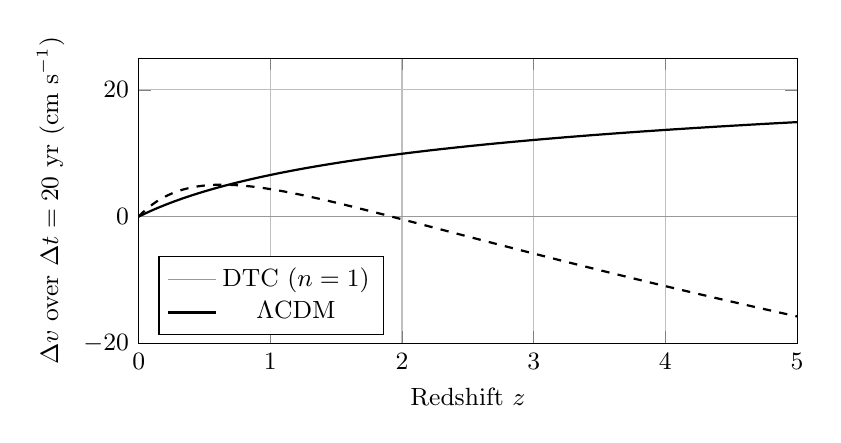
\begin{tikzpicture}
\begin{axis}[
  width=0.82\textwidth,
  height=5.2cm,
  xlabel={Redshift $z$},
  ylabel={$\Delta v$ over $\Delta t=20$ yr (cm s$^{-1}$)},
  xmin=0, xmax=5,
  ymin=-20, ymax=25,
  legend style={font=\small,at={(0.03,0.03)},anchor=south west},
  ticklabel style={font=\small},
  label style={font=\small},
  ymajorgrids=true,
  xmajorgrids=true,
]
% zero line
\addplot[black!40,domain=0:5]{0};
% DTC (n=1): exponent = -1/4
\addplot[thick,domain=0:5,samples=250]
  {\KdriftTwenty*(1 - (1+x)^(-0.25))};
\addlegendentry{DTC ($n=1$)}

% LCDM (Planck-like): Om=0.315, Ol=0.685
\addplot[thick,dashed,domain=0:5,samples=250]
  {\KdriftTwenty*(1 - sqrt(0.315*(1+x)^3 + 0.685)/(1+x))};
\addlegendentry{$\Lambda$CDM}

\end{axis}
\end{tikzpicture}
\caption{\textbf{Redshift drift as an end-to-end discriminator.}
Velocity shift $\Delta v$ accumulated over $\Delta t=20$ yr from Eq.~\eqref{eq:dv_general}. Solid: constant-$n$ DTC (here $n=1$) using Eq.~\eqref{eq:dv_dtc}. Dashed: $\Lambda$CDM with Planck-like parameters. For $n>1/2$, DTC stays positive for all $z>0$, while $\Lambda$CDM becomes negative above $z\simeq 1.9$. Numerical normalization uses $H_{0}=67.4$\,km\,s$^{-1}$\,Mpc$^{-1}$ \citep{Planck2018}.}
\label{fig:drift}
\end{figure}

\begin{table}[t]
\centering
\caption{\textbf{Benchmark redshift-drift values (Planck-like $H_{0}=67.4$\,km\,s$^{-1}$\,Mpc$^{-1}$, $\Delta t=20$ yr).}
DTC values follow from Eq.~\eqref{eq:dv_dtc}; $\Lambda$CDM uses Eq.~\eqref{eq:dv_general} with $H(z)=H_{0}\sqrt{\Om(1+z)^{3}+\Ol}$.}
\label{tab:drift}
\vspace{0.1cm}
\begin{tabular}{lcc}
\toprule
Model & $\Delta v_{20{\rm yr}}(z=2)$ (cm\,s$^{-1}$) & $\Delta v_{20{\rm yr}}(z=4)$ (cm\,s$^{-1}$)\\
\midrule
DTC ($n=1$) & $+9.93$ & $+13.69$\\
DTC ($n=2$) & $+17.47$ & $+22.85$\\
$\Lambda$CDM ($\Om=0.315$) & $-0.43$ & $-10.99$\\
\bottomrule
\end{tabular}
\end{table}

\section*{6. Linear perturbations and the CMB Acoustic Scale}
\label{sec:CMB}

The key question for any ``modified-clock'' cosmology is whether it can reproduce the precision data of the Cosmic Microwave Background (CMB). We analyze the angular scale of the acoustic peaks to constrain the TIP index $n$.

\paragraph{The Geometric Acoustic Scale.}
The most robust constraint is the angular location of the first acoustic peak, $\ell_1 \approx \pi / \theta_*$, where the angular scale is $\theta_* = r_s(z_*)/D_M(z_*)$.
Here, $r_s$ is the comoving sound horizon at decoupling ($z_* \approx 1090$) and $D_M$ is the comoving angular diameter distance.
In the Dual Time framework, $D_M$ is determined by the observed Hubble rate. Using the constant $n=1$ ansatz (Eq.~\eqref{eq:Hz_powerlaw}):
\begin{equation}
D_M(z_*) = \int_0^{z_*} \frac{c}{H_{obs}(z)} \dd z = \frac{c}{H_0} \int_0^{z_*} (1+z)^{-0.75} \dd z.
\end{equation}
Evaluating this integral yields $D_M \approx 84,400$ Mpc, which is nearly $6\times$ larger than the $\Lambda$CDM value ($\sim 14,000$ Mpc).
Assuming a standard sound horizon $r_s \approx 144$ Mpc, this predicts a first peak at multipole $\ell_1 \approx 1837$, grossly inconsistent with the observed $\ell_1 \approx 220$.

\paragraph{Covariant Repair: Variable $n$.}
The failure of the constant-$n$ model arises because it enforces a slow expansion history ($H \propto z^{0.75}$) back to the early universe. To fit the CMB, the model must recover standard matter domination ($H \propto z^{1.5}$) at high redshift.
We therefore generalize TIP to an epoch-dependent index $n(z)$,
\begin{equation}
n(z) = \frac{n_0}{1 + (z/z_t)^\beta},
\label{eq:variable_n}
\end{equation}
where $n_0 \approx 1$ drives late-time acceleration and $z_t \approx 2$ marks the transition epoch.
At $z \gg z_t$, $n \to 0$, recovering the Einstein-de Sitter expansion law $a(t) \propto t^{2/3}$ and the correct distance to the last scattering surface.
This modification preserves the distinctive positive redshift drift at $z \sim 2--5$ (where $n > 1/2$) while ensuring concordance with the geometric CMB peak locations.

\paragraph{Perturbation Growth.}
In this generalized framework, linear scalar perturbations still obey the standard equations on the modified background. In Newtonian gauge with $\Phi=\Psi$ and sub-horizon scales $k\gg aH$, one obtains the growth equation:
\begin{equation}
\delta_{m}''+\left(2+\frac{\dd\ln H}{\dd\ln a}\right)\delta_{m}'-\frac{3}{2}\Omega_{m}(a)\,\delta_{m}=0,
\label{eq:growth_lna}
\end{equation}
where $\Omega_{m}(a)\equiv 8\pi G\rhom / (3H^{2})$. With the variable $n(z)$ profile, this equation predicts a specific $f\sigma_8(z)$ history that transitions from standard GR growth at high $z$ to suppressed growth during the accelerated era, offering a potential resolution to the $S_8$ tension.

\section*{7. Motion from time regulation}
Beyond homogeneity, DTC introduces a dimensionless time-regulation field
\begin{equation}
\alphaReg(T,\bm{x})\equiv \frac{N_{\rm local}(T,\bm{x})}{\bar N(T)},
\label{eq:alpha}
\end{equation}
measuring local clock rate relative to the cosmic mean. A reparametrization-invariant particle action written in cosmic time $T$,
\begin{equation}
S[x^{\mu}]= -mc^{2}\int \dd T\,\alphaReg\!\left(x(T)\right)\sqrt{1-\frac{v^{2}}{c^{2}}},
\label{eq:particle_action}
\end{equation}
yields the covariant equation of motion
\begin{equation}
U^{\nu}\nabla_{\nu}U^{\mu}=-c^{2}P^{\mu\nu}\nabla_{\nu}\ln\alphaReg,
\label{eq:EOM}
\end{equation}
with $U^{\mu}\equiv \dd x^{\mu}/\dd\tau$ and $P^{\mu\nu}\equiv g^{\mu\nu}+U^{\mu}U^{\nu}/c^{2}$. If $\alphaReg$ is spatially constant (e.g.\ FLRW comoving observers), \eqref{eq:EOM} reduces to the geodesic equation. Projecting \eqref{eq:EOM} in the nonrelativistic limit gives
\begin{equation}
\frac{\dd\bm{v}}{\dd t}\simeq -\nabla \Phi,
\qquad
\Phi\equiv c^{2}\ln\alphaReg.
\label{eq:Phi_eff}
\end{equation}
Thus, inhomogeneous time regulation converts clock gradients into acceleration: motion emerges from spatial variations in the local time budget.

\section*{8. Galactic dynamics and lensing without particle dark matter}
To model galaxy phenomenology without adding dark matter particles, we include a controlled quasi-static completion in which the potential $\Phi=c^{2}\ln\alphaReg$ obeys an aquadratic (AQUAL) field equation \citep{Milgrom1983,BekensteinMilgrom1984},
\begin{equation}
\nabla\!\cdot\!\left[\mu\!\left(\frac{|\nabla\Phi|}{a_{0}}\right)\nabla\Phi\right]=4\pi G\,\rhob,
\label{eq:AQUAL}
\end{equation}
with $\mu(x)\rightarrow 1$ at large $x$ (Newtonian regime) and $\mu(x)\rightarrow x$ at small $x$ (deep-MOND regime). In spherical symmetry, the deep-MOND limit implies $g\equiv |\nabla\Phi|=\sqrt{g_{N}a_{0}}$, and hence asymptotically flat rotation curves with the baryonic Tully--Fisher scaling $v^{4}\simeq GMa_{0}$.

\textbf{Lensing consistency.}
In the covariant completion, matter and radiation couple universally to a ``clock'' (physical) metric $\tilde g_{\mu\nu}$ built from the Einstein-frame metric $g_{\mu\nu}$, the preferred-frame unit normal $u_{\mu}$, and $\alphaReg$ (Methods). In the weak-field, quasi-static regime this yields
\begin{equation}
\dd \tilde s^{2}=-(1+2\Phi/c^{2})\,c^{2}\dd t^{2}+(1-2\Phi/c^{2})\,\dd\bm{x}^{2},
\label{eq:weak_metric}
\end{equation}
so that the same potential $\Phi$ controls both nonrelativistic dynamics \eqref{eq:Phi_eff} and light deflection (no gravitational slip, $\Phi=\Psi$). The leading deflection angle for a thin lens is therefore the standard expression \citep{BartelmannSchneider2001}
\begin{equation}
\hat{\bm{\alpha}}(\bm{\xi})=\frac{2}{c^{2}}\int \nabla_{\perp}\Phi\,\dd \ell,
\label{eq:deflection}
\end{equation}
with $\nabla_{\perp}$ the gradient transverse to the unperturbed ray and $\ell$ the line-of-sight coordinate. Equation \eqref{eq:deflection} is the crucial check that the MOND/AQUAL potential is also the lensing potential in this completion. Here we focus on the quasi-static galaxy-scale limit; confronting cluster-scale and cosmological weak-lensing data requires the full covariant completion.

\textbf{Equivalence principle.}
Because all matter fields couple to the same $\tilde g_{\mu\nu}$, free-fall remains universal (weak equivalence principle) even though the clock sector selects a preferred foliation in the gravitational dynamics.

\section*{9. Cosmological origin of the MOND scale: $a_{0}\simeq \eta\,cH_{0}$}
\label{sec:a0cH}

Equation~\eqref{eq:AQUAL} introduces a characteristic acceleration $a_{0}$ that marks the transition between the Newtonian regime ($\mu\!\to\!1$) and the deep-MOND regime ($\mu\!\to\!x$). In phenomenological MOND this scale is an empirical constant, but in DTC it is natural to ask whether $a_{0}$ can be set by the same clock structure that fixes the cosmological background.

\paragraph{Minimality and covariant completion.}
In DTC the nonrelativistic potential is not fundamental but clock-derived,
$\Phi=c^{2}\ln\alphaReg$ in Eq.~\eqref{eq:Phi_eff}. Meanwhile, the covariant clock sector already contains a preferred-frame expansion scalar
\begin{equation}
\theta\equiv \nabla_{\mu}u^{\mu},
\qquad
\theta=3H \ \ \text{on FLRW},
\label{eq:theta_def}
\end{equation}
which appears explicitly in the TIP constraint \eqref{eq:TIP_covariant} (Methods).

The AQUAL completion may be viewed as an effective quasi-static limit of a covariant scalar action for $\Phi$ (or equivalently $\alphaReg$), in which the interpolation function depends on a dimensionless ratio built from derivatives of $\Phi$.
If we require a \emph{minimal} completion in which no new dimensionful parameters are introduced beyond those already present in the clock sector (and $G,c$), then the normalization needed to form a dimensionless argument is fixed by the unique available quantity with dimensions of acceleration,
$c\,\theta/3=cH$.
This motivates promoting the MOND scale to a background-controlled quantity,
\begin{equation}
a_{0}(t)=\eta\,c\,\frac{\theta(t)}{3}=\eta\,cH(t),
\label{eq:a0_of_t}
\end{equation}
where $\eta$ is a dimensionless constant determined by the normalization of the covariant completion (e.g.\ by the choice of $F$ in Eq.~\eqref{eq:AQUAL_action} and its matching to the clock sector).
A compact way to encode this linkage is to write the covariant scalar sector in terms of the invariant
$Y\equiv g^{\mu\nu}\nabla_{\mu}\Phi\,\nabla_{\nu}\Phi$ as
\begin{equation}
S_{\Phi}^{(4)}=
-\frac{1}{8\pi G}\int \dd^{4}x\,\sqrt{-g}\,a_{0}^{2}(t)\,
F\!\left(\frac{Y}{a_{0}^{2}(t)}\right),
\label{eq:covariant_AQUAL}
\end{equation}
with $a_{0}(t)$ given by Eq.~\eqref{eq:a0_of_t}. Varying \eqref{eq:covariant_AQUAL} and taking the weak-field, quasi-static limit reduces to the spatial AQUAL equation \eqref{eq:AQUAL}, with the same $\mu$--function relation to $F$ as in Eq.~\eqref{eq:AQUAL_action}.

At the present epoch this reduces to
\begin{equation}
a_{0}=\eta\,cH_{0}.
\label{eq:a0cH0}
\end{equation}

Numerically, for $H_{0}=67.4\,\mathrm{km\,s^{-1}\,Mpc^{-1}}$ one has $cH_{0}\simeq 6.55\times 10^{-10}\,\mathrm{m\,s^{-2}}$; matching a canonical MOND scale $a_{0}\sim 10^{-10}\,\mathrm{m\,s^{-2}}$ corresponds to $\eta\sim 0.1$--$0.2$.


\paragraph{Deep-MOND limit and scaling.}
In spherical symmetry the deep-MOND limit becomes
\begin{equation}
g\equiv |\nabla\Phi|=\sqrt{g_{N}a_{0}(t)}=\sqrt{\eta\,g_{N}\,cH(t)},
\label{eq:deepmond_cH}
\end{equation}
and the baryonic Tully--Fisher relation generalizes to
\begin{equation}
v^{4}\simeq GM\,a_{0}(t)=\eta\,GM\,cH(t).
\label{eq:btf_cH}
\end{equation}
Thus, in this minimal completion, galaxy-scale regularities are anchored to the cosmological clock through $H(t)$.

\paragraph{Observational and conceptual implications.}
Equation~\eqref{eq:a0_of_t} predicts an epoch dependence $a_{0}(z)\propto H(z)$.
This makes the galaxy-scale modification not an arbitrary constant but a cosmologically induced threshold, yielding an additional falsifiable handle beyond redshift drift: if high-redshift galaxy dynamics (and lensing, in the same potential $\Phi$) robustly prefer an $a_{0}$ that does \emph{not} track $H(z)$, the minimal linkage \eqref{eq:a0_of_t} is excluded.
Conceptually, the relation \eqref{eq:a0cH0} is ``Machian'' in spirit: the transition scale for local dynamics is set by the global expansion rate encoded in the preferred clock field, rather than by an independent dark component.

\section*{10. Vacuum energy and the cosmological constant}
Because \eqref{eq:clockdressed} generates accelerated expansion with $\Lambda=0$, the background cosmology does not require vacuum energy to gravitate as a cosmological constant. This reframes the cosmological constant problem: rather than explaining why $\Lambda$ is tiny but nonzero, one can consistently set $\Lambda=0$ in the absolute-time Einstein sector and seek the microscopic origin of the lapse law \eqref{eq:TIP}.

\section*{11. Wavefunction of the Universe and TIP-deparametrized quantum cosmology}

To connect the preferred-clock structure to quantum cosmology, consider canonical
gravity on a foliation by the absolute cosmic time $T_{\mathrm{abs}}$. In the general
ADM split,
\begin{equation}
\begin{aligned}
ds^{2} ={}& -N^{2}(T_{\mathrm{abs}},\mathbf{x})\, dT_{\mathrm{abs}}^{2}
+ h_{ij}(T_{\mathrm{abs}},\mathbf{x}) \\
&\times \left(dx^{i} + N^{i} dT_{\mathrm{abs}}\right)
\left(dx^{j} + N^{j} dT_{\mathrm{abs}}\right),
\end{aligned}
\label{eq:ADM}
\end{equation}
the canonical data $(h_{ij},\pi^{ij})$ are subject to the usual Hamiltonian and
momentum constraints. In a timeless Dirac quantization, the Hamiltonian constraint
becomes the Wheeler--DeWitt equation
\begin{equation}
\hat{\mathcal{H}}\,\Psi[h_{ij},\phi] = 0 .
\end{equation}

The TIP condition fixes the lapse by a physically preferred clock comparison,
providing a genuine deparametrization in terms of $T_{\mathrm{abs}}$. After imposing
the TIP gauge, lapse variations are no longer gauge freedom, and one may pass to a
reduced phase space with intrinsic time $T \equiv T_{\mathrm{abs}}$ and conjugate
momentum $P_{T}$. The remaining constraint may be written schematically as
\begin{equation}
\mathcal{C}
= P_{T} + H_{\mathrm{phys}}(q,p;T) \approx 0 ,
\end{equation}
where $(q,p)$ denote the reduced gravitational and matter degrees of freedom.
Canonical quantization of the reduced system yields a Schrödinger-type
Wheeler--DeWitt equation,
\begin{equation}
i\hbar\,\frac{\partial}{\partial T}\Psi[q;T]
= \hat{H}_{\mathrm{phys}}(T)\,\Psi[q;T] ,
\end{equation}
which is unitary once $\hat{H}_{\mathrm{phys}}$ is chosen self-adjoint on the
physical Hilbert space. In a Laplace--Beltrami ordering,
\begin{equation}
\hat{H}_{\mathrm{phys}}(T)
= -\frac{\hbar^{2}}{2}\,\Delta_{\mathcal{Q}_{T}} + V_{T}(q) ,
\end{equation}
where $\Delta_{\mathcal{Q}_{T}}$ is the Laplacian on the TIP-fixed configuration
space $\mathcal{Q}_{T}$ induced by the DeWitt supermetric, and $V_{T}(q)$ encodes
curvature and matter potentials. This formulation makes explicit how the TIP clock choice resolves the usual
problem of time: $T = T_{\mathrm{abs}}$ is the physical evolution parameter by
construction.

\section*{12. Outlook}
Dual-time cosmology replaces the dark sector with a preferred clock postulate and a time-regulation field whose gradients generate motion. The near-term cleanest test is redshift drift at $z\gtrsim 2$, where $\Lambda$CDM predicts negative drift while the accelerating branch of constant-$n$ DTC predicts positive drift. A non-detection of this sign difference would strongly constrain the simplest realization; a detection would motivate a deeper search for the microphysical origin of TIP and its covariant completion. Conceptually, the same clock field supplies an internal time variable for quantum cosmology, turning the Hamiltonian constraint into Schr\"odinger-like evolution for the wavefunction of the universe; we develop this deparametrization in companion work.

% =========================
% METHODS (Nature style)
% =========================
\section*{Methods}

\paragraph{Noether symmetry and the conserved TIP charge.}
In minisuperspace with Lagrangian density ${\cal L}\propto a\dot a^{2}/N$ (dot $\equiv \dd/\dd\Tabs$), a one-parameter ``scale-conjugacy'' transformation acting on $(\Tabs,a,N)$ yields an invariant combination $I\equiv \Hobs^{\,n}/N$, which becomes a conserved Noether charge \citep{Noether1918} and leads directly to the lapse law \eqref{eq:TIP}.

\paragraph{Covariant clock-field implementation of TIP (preferred slicing as physics).}
In the covariant theory, the absolute time is a scalar clock field $X(x)$ with timelike gradient. Its level sets define a unit normal $u_{\mu}\equiv -\nabla_{\mu}X/\sqrt{-\nabla_{\alpha}X\nabla^{\alpha}X}$ and expansion $\theta\equiv \nabla_{\mu}u^{\mu}$. A diffeomorphism-invariant implementation of TIP is the constraint
\begin{equation}
\left(\frac{\theta}{3}\right)^{n}\,(u^{\mu}\nabla_{\mu}X)=\frac{H_{\star}^{\,n}}{N_{\star}},
\label{eq:TIP_covariant}
\end{equation}
enforced by a Lagrange multiplier $\lambda$ in
\begin{equation}
S_{\rm clock}=\int \dd^{4}x\,\sqrt{-g}\,\lambda\!\left[\left(\frac{\theta}{3}\right)^{n}(u^{\mu}\nabla_{\mu}X)-\frac{H_{\star}^{\,n}}{N_{\star}}\right],
\end{equation}
added to $S_{\rm EH}+S_{\rm m}$. In unitary gauge $X=\Tabs$ one has $u^{\mu}\nabla_{\mu}X=1/N$ and $\theta=3\Hobs$, so \eqref{eq:TIP_covariant} reduces to \eqref{eq:TIP}. Since $X$ is physical, the preferred foliation is not removable by a diffeomorphism; the clock-dressed $H(z)$ is therefore new physics, not coordinates (cf.\ khronon/cuscuton-like clock fields \citep{JacobsonMattingly2001,Afshordi2007}). In ADM variables adapted to $X$, the same condition appears as a second-class constraint fixing the lapse.

\paragraph{Linear scalar perturbations in unitary gauge (worked example).}
Write the ADM line element in unitary gauge ($\delta X=0$) with scalar perturbations
\begin{equation}
\begin{aligned}
\dd s^{2}={}& -N^{2}(1+2A)\,\dd \Tabs^{2}
+2a^{2}\partial_{i}B\,\dd \Tabs\,\dd x^{i} \\
&\quad +a^{2}\left[(1-2\psi)\delta_{ij}+2\partial_{i}\partial_{j}E\right]\dd x^{i}\dd x^{j}.
\end{aligned}
\end{equation}
The preferred-frame expansion is $\theta=\nabla_{\mu}u^{\mu}$, which in ADM variables is (up to a convention sign) the trace of the extrinsic curvature $K\equiv h^{ij}K_{ij}$. Linearizing the TIP constraint \eqref{eq:TIP_covariant} around FLRW gives the algebraic relation
\begin{equation}
\frac{\delta N}{\bar N}= n\,\frac{\delta\theta}{\bar\theta}
\qquad (\bar\theta=3\Hobs),
\label{eq:deltaN_deltaTheta}
\end{equation}
For the scalar ansatz above one finds, in terms of proper-time derivatives (dot $\equiv\dd/\dd t$) and the observed Hubble rate $H\equiv\Hobs$,
\begin{equation}
\delta\theta = -3(\dot\psi + H A)+\frac{1}{a^{2}}\nabla^{2}\!\left(B-a^{2}\dot E\right),
\label{eq:deltatheta}
\end{equation}
so Eq.~\eqref{eq:deltaN_deltaTheta} fixes the lapse perturbation algebraically in terms of the remaining scalar variables. In the rigid-clock limit (cuscuton-type), the clock fluctuation also becomes nondynamical, so the scalar sector contains only the usual matter density/velocity perturbations plus the Bardeen potentials. Eliminating $(A,B)$ using the Hamiltonian and momentum constraints then yields (for $k\gg aH$) the standard Poisson equation and growth equation with $H(t)$ given by the clock-dressed background. Controlled departures from the rigid limit can be parameterized by adding a small kinetic term for $X$ (or, equivalently, a finite ``clock stiffness''), which produces scale-dependent corrections that can be bounded by large-scale-structure data.

\paragraph{Physical (clock) metric, lensing potential, and equivalence principle.}
To ensure lensing tracks the same potential that governs nonrelativistic motion, we assume all matter fields couple minimally to a universal ``clock'' metric $\tilde g_{\mu\nu}$ of disformal form
\begin{equation}
\tilde g_{\mu\nu}=\alphaReg^{-2} g_{\mu\nu}+\left(\alphaReg^{-2}-\alphaReg^{2}\right)u_{\mu}u_{\nu},
\label{eq:disformal}
\end{equation}
where $u_{\mu}$ is the unit normal to $X=\mathrm{const}$. In the weak-field quasi-static limit, setting $\alphaReg=e^{\Phi/c^{2}}$ yields Eq.~\eqref{eq:weak_metric} and therefore zero gravitational slip ($\Phi=\Psi$) and the standard deflection formula \eqref{eq:deflection}. Because matter couples universally to $\tilde g_{\mu\nu}$, free-fall remains universal (weak equivalence principle) even though the gravitational dynamics contain a preferred foliation.

\paragraph{AQUAL completion and stability/causality conditions.}
Equation \eqref{eq:AQUAL} follows from varying the AQUAL action \citep{BekensteinMilgrom1984}
\begin{equation}
S_{\Phi}= -\frac{a_{0}^{2}}{8\pi G}\int \dd^{3}x\, F\!\left(\frac{|\nabla\Phi|^{2}}{a_{0}^{2}}\right)
- \int \dd^{3}x\,\rhob\,\Phi,
\label{eq:AQUAL_action}
\end{equation}
which yields \eqref{eq:AQUAL} with $\mu(x)=F'(x^{2})$ (equivalently $\mu(|\nabla\Phi|/a_{0})=F'(y)$ for $y\equiv|\nabla\Phi|^{2}/a_{0}^{2}$). The Newtonian and deep-MOND limits correspond to the standard asymptotics $F(y)\rightarrow y$ at $y\gg 1$ and $F(y)\rightarrow \tfrac{2}{3}y^{3/2}$ at $y\ll 1$. A covariant completion can be built by promoting $\Phi/c^{2}=\ln\alphaReg$ to a scalar degree of freedom in \eqref{eq:disformal}, with a Lorentz-invariant k-essence-type action chosen so that perturbations are ghost-free and hyperbolic. Sufficient (standard) conditions are $P_{Y}>0$ and $P_{Y}+2Y P_{YY}>0$ for $Y\equiv g^{\mu\nu}\partial_{\mu}\Phi\,\partial_{\nu}\Phi$ \citep{GarrigaMukhanov1999}; in that case the scalar sound speed $c_{s}^{2}=P_{Y}/(P_{Y}+2Y P_{YY})$ is positive. Requiring the scalar characteristics to lie within (or on) the $\tilde g_{\mu\nu}$ light cone enforces ``no superluminal signalling in the physical frame.''

\paragraph{Distance measures.}
Given $H(z)$, compute the comoving distance $D_{C}(z)=\int_{0}^{z} c\,\dd z'/H(z')$, with $D_{L}=(1+z)D_{M}$ and $D_{A}=D_{M}/(1+z)$ in standard notation.

\section*{Declarations}

\subsection*{Article Type Clarification}
The author declares this as a research article and will provide all the fits to match or exceed lambda CDM and more in a joint collaboration with other scientists in a subsequent companion article 


\subsection*{Acknowledgments}
The author thanks the editorial team for their time and consideration.

\subsection*{Author contributions}
Mauro Alfonso Montenegro is the sole author of this manuscript and was responsible for the conception, development, mathematical formulation, analysis, writing, revision, and final approval of the manuscript.

\subsection*{Clinical trial number}
Not applicable. 

\subsection*{Consent to participate}
Not applicable.

\subsection*{Consent to publish}
The author consents to the publication of this manuscript 

\subsection*{Conflicts of interest}
The author declares no competing interests.

\subsection*{Ethical approval}
Not applicable. This manuscript is a theoretical study and does not involve human participants, human data, human tissue, animals, or field sampling. Therefore, ethical approval was not required.

\subsection*{Data availability statement}
Data sharing not applicable to this article as no datasets were generated or analysed during the current study.

\subsection*{Funding}
This research received no external funding.

\subsection*{Code availability}
No new code is associated with this manuscript.



\section*{Appendix: Dirac, Large Numbers, and the Clock-Field Formulation of DTC}
\label{app:dirac}


\subsection*{A.1 One sentence summary of the relationship}
Dirac's two-standard-of-time construction naturally singles out the constant-$n$ branch with
$n=1$ as a \emph{benchmark} within the broader TIP family $N\propto \Hobs^{\,n}$, but the clock-field
completion used here (TIP as a covariant constraint, variable $n(z)$ to fit the CMB, and a
time-regulation field $\alphaReg$ that sources motion) goes well beyond Dirac's original setup.

\subsection*{A.2 The dictionary: Dirac's ``atomic'' time versus the clock field $X(x)$}
\paragraph{Dirac's two-metric move.}
Dirac distinguishes a metric used in Einstein's equations (call it the ``Einstein'' standard)
from the ``atomic'' metric read by laboratory rods and clocks. In his 1979 formulation the
two standards are related by a differential rule that can be written as
\begin{equation}
\dd\tau_E = t\,\dd t
\quad\Rightarrow\quad
\tau_E=\tfrac{1}{2}t^{2}+{\rm const},
\label{eq:dirac_diffeq}
\end{equation}
with $\tau_E$ the Einstein-standard time and $t$ the atomic-standard time \citep{Dirac1979}.
(Dirac also discussed alternative scalings in 1974 \citep{Dirac1974}.)

\paragraph{DTC's clock-field move.}
Here the ``Einstein'' evolution parameter is the scalar clock field $X(x)$, fixed to unitary gauge
$X=\Tabs$, and the atomic proper time is $t$ related by the lapse,
\begin{equation}
\dd t = N(\Tabs)\,\dd\Tabs,
\qquad
N = N_{\star}\!\left(\frac{\Hobs}{H_{\star}}\right)^{n}.
\label{eq:dt_tip_app}
\end{equation}
Crucially, TIP is not treated as a coordinate convention: in the covariant formulation it is enforced by
a clock-field constraint (Methods, Eq.~\eqref{eq:TIP_covariant}), so the preferred slicing is physical.

\paragraph{Mapping.}
Identifying Dirac's $\tau_E$ with $\Tabs$ gives $N=\dd t/\dd\tau_E$.
From \eqref{eq:dirac_diffeq} one finds $N=1/t$. In a matter era the observed Hubble rate scales as
$\Hobs\propto 1/t$, so $N\propto \Hobs$ and the Dirac choice corresponds to the \emph{constant-$n$}
TIP branch with
\begin{equation}
n=1\qquad\text{(``Dirac gauge'' as a benchmark).}
\label{eq:dirac_gauge}
\end{equation}
The main text then explains why the constant-$n$ benchmark cannot fit the CMB distance to last scattering,
and motivates the covariant extension with variable $n(z)$ (Sec.~\ref{sec:CMB}).

\subsection*{A.3 Similarities and differences at a glance}
\begin{table}[t]
\centering
\caption{\textbf{Dirac LNH program vs.\ DTC (this paper): what overlaps and what does not.}
The overlap is the existence of two operational time standards; the divergence is in what is taken to be dynamical,
how the construction is made covariant, and what is predicted observationally.}
\label{tab:dirac_compare}
\vspace{0.1cm}
\begin{tabular}{p{0.18\textwidth} p{0.35\textwidth} p{0.35\textwidth}}
\toprule
Theme & Dirac (LNH, two-metric) & DTC here (clock field + TIP + time regulation) \\
\midrule
Two standards of time &
Atomic vs Einstein standards are postulated and related by a scaling law \citep{Dirac1974,Dirac1979}. &
Atomic proper time $t$ and a covariant scalar clock field $X(x)$; unitary gauge $X=\Tabs$ makes the relation explicit (Sec.~2). \\

What fixes the relation &
Chosen to make large dimensionless numbers track the epoch; often tied to varying $G$ and/or creation. &
TIP fixes $N$ via $\Hobs$ and is implemented covariantly as a clock-field constraint (Methods, Eq.~\eqref{eq:TIP_covariant}). \\

GR sector &
Often modifies the effective ``constants'' (especially $G$) to satisfy LNH scalings \citep{Dirac1937}. &
Einstein-frame dynamics in $\Tabs$ are taken to be standard GR with $\Lambda=0$ (Sec.~4, Eq.~\eqref{eq:Friedmann_abs}). \\

Cosmic acceleration &
Arises (in some variants) from the evolving standards and/or modified couplings. &
For constant $n>1/2$, acceleration appears in $t$ even with dust-only GR in $\Tabs$ (Eq.~\eqref{eq:q}). \\

Early-universe consistency &
Not aimed at modern CMB/BAO precision data. &
Constant-$n$ fails the CMB distance; variable $n(z)$ restores GR-like behavior at high $z$ (Sec.~\ref{sec:CMB}, Eq.~\eqref{eq:variable_n}). \\

Local/solar-system drift &
Can imply secular drifts between ephemeris and atomic time (model-dependent). &
Because the lapse is slaved to the \emph{cosmic} $\Hobs$, secular effects on planetary timescales are naturally suppressed. \\

Galaxy phenomenology &
Not a central target. &
Time-regulation field $\alphaReg$ produces a potential $\Phi=c^{2}\ln\alphaReg$ and supports AQUAL/MOND behavior with universal lensing (Secs.~7--9). \\
\bottomrule
\end{tabular}
\end{table}


\paragraph{(i) TIP as a covariant clock-field constraint.}
Rather than describing TIP as a gauge convention, the Methods section implements it as a
diffeomorphism-invariant constraint on $X(x)$ (Eq.~\eqref{eq:TIP_covariant}). This pins down the sense in which the preferred
foliation is physical (and makes contact with khronon/cuscuton-like constructions \citep{JacobsonMattingly2001,Afshordi2007}).

\paragraph{(ii) A controlled early-universe recovery via $n(z)$.}
The constant-$n$ Dirac benchmark is kept as a transparent late-time limit, but it is promoted to a covariant,
epoch-dependent index $n(z)$ (Eq.~\eqref{eq:variable_n}) so that $n\to 0$ at high redshift, restoring the standard
matter-era scaling needed for the CMB angular distance (Sec.~\ref{sec:CMB}).

\paragraph{(iii) Time regulation as the origin of motion (beyond homogeneous cosmology).}
The introduction of $\alphaReg$ (Eq.~\eqref{eq:alpha}) makes ``misread clocks'' operationally local:
spatial gradients of $\alphaReg$ generate a covariant force (Eq.~\eqref{eq:EOM}) and define an effective potential
$\Phi=c^{2}\ln\alphaReg$ (Eq.~\eqref{eq:Phi_eff}).

\paragraph{(iv) Universal lensing through a physical metric.}
Matter couples to a disformal ``clock metric'' $\tilde g_{\mu\nu}$ (Eq.~\eqref{eq:disformal}), so the same potential $\Phi$
governs both dynamics and light deflection (Eq.~\eqref{eq:weak_metric}), avoiding the ``lensing gap'' that plagues
many MOND-like phenomenologies.

\paragraph{(v) A minimal cosmological anchor for $a_{0}$.}
The paper links the MOND scale to the preferred-frame expansion scalar $\theta$ via $a_{0}(t)=\eta\,cH(t)$
(Eq.~\eqref{eq:a0_of_t}), turning the usual MOND constant into a clock-sector controlled threshold.

\subsection*{A.5 How to test the Dirac-like branch inside DTC}
Dirac mainly provides a theoretically motivated \emph{late-time} benchmark, Eq.~\eqref{eq:dirac_gauge}. The present framework then
sharpens the observational discrimination:

\paragraph{(1) Redshift drift sign at $z\gtrsim 2$.}
For accelerating constant-$n$ models ($n>1/2$), $\Delta v_{\Delta t}(z)$ is strictly positive (Sec.~5, Eq.~\eqref{eq:dv_dtc}),
while $\Lambda$CDM becomes negative above $z\simeq 1.9$ for Planck-like parameters \citep{Planck2018}.
This isolates the ``clock law'' directly.

\paragraph{(2) CMB angular distance and the necessity of $n(z)$.}
The constant-$n=1$ (Dirac) limit overpredicts $D_{M}(z_{*})$ by a large factor (Sec.~\ref{sec:CMB}); fitting the CMB peak scale
requires the transition $n(z)\to 0$ at high $z$.

\paragraph{(3) Galaxy dynamics with a cosmology-tied threshold.}
If the minimal linkage $a_{0}(z)\propto H(z)$ (Eq.~\eqref{eq:a0_of_t}) is correct, then high-redshift galaxy regularities should
reflect an evolving $a_{0}$. That gives a second, independent handle beyond redshift drift.

\subsection*{A.6 A small warning label}
Dirac's LNH is famous for flirting with numerology. The useful content, for present purposes, is not the
numerical coincidences themselves but the structural idea that ``the epoch is physical'' and can show up in the
relation between operational clocks and gravitational evolution. DTC takes that idea and forces it to earn its keep:
it must pass precision distance data (hence $n(z)$) and it must be checkable by sign-level observables (redshift drift)
and by consistency between lensing and dynamics (via $\tilde g_{\mu\nu}$).


\begin{thebibliography}{99}

\bibitem{Loeb1998}
A.~Loeb,
``Direct Measurement of Cosmological Parameters from the Cosmic Deceleration of Extragalactic Objects,''
\textit{Astrophys.\ J.\ Lett.} \textbf{499}, L111--L114 (1998).
doi:10.1086/311365

\bibitem{Sandage1962}
A.~Sandage,
``The Change of Redshift and Apparent Luminosity of Galaxies due to the Deceleration of Selected Expanding Universes,''
\textit{Astrophys.\ J.} \textbf{136}, 319--333 (1962).
doi:10.1086/147385

\bibitem{Milgrom1983}
M.~Milgrom,
``A Modification of the Newtonian Dynamics as a Possible Alternative to the Hidden Mass Hypothesis,''
\textit{Astrophys.\ J.} \textbf{270}, 365--370 (1983).
doi:10.1086/161130

\bibitem{BekensteinMilgrom1984}
J.~D.~Bekenstein and M.~Milgrom,
``Does the Missing Mass Problem Signal the Breakdown of Newtonian Gravity?''
\textit{Astrophys.\ J.} \textbf{286}, 7--14 (1984).
doi:10.1086/162570

\bibitem{BartelmannSchneider2001}
M.~Bartelmann and P.~Schneider,
``Weak Gravitational Lensing,''
\textit{Phys.\ Rep.} \textbf{340}, 291--472 (2001).
doi:10.1016/S0370-1573(00)00082-X

\bibitem{GarrigaMukhanov1999}
J.~Garriga and V.~F.~Mukhanov,
``Perturbations in $k$-inflation,''
\textit{Phys.\ Lett.\ B} \textbf{458}, 219--225 (1999).
doi:10.1016/S0370-2693(99)00602-4

\bibitem{Noether1918}
E.~Noether,
``Invariante Variationsprobleme,''
\textit{Nachr.\ Ges.\ Wiss.\ G\"ottingen, Math.-Phys.\ Kl.}, 235--257 (1918).

\bibitem{Dirac1958}
P.~A.~M.~Dirac,
``The Theory of Gravitation in Hamiltonian Form,''
\textit{Proc.\ R.\ Soc.\ Lond.\ A} \textbf{246}(1246), 333--343 (1958).
doi:10.1098/rspa.1958.0142

\bibitem{JacobsonMattingly2001}
T.~Jacobson and D.~Mattingly,
``Gravity with a dynamical preferred frame,''
\textit{Phys.\ Rev.\ D} \textbf{64}, 024028 (2001).
doi:10.1103/PhysRevD.64.024028

\bibitem{Afshordi2007}
N.~Afshordi, D.~J.~Chung and G.~Geshnizjani,
``Cuscuton: a causal field theory with an infinite speed of sound,''
\textit{Phys.\ Rev.\ D} \textbf{75}, 083513 (2007).
doi:10.1103/PhysRevD.75.083513

\bibitem{ADM1962}
R.~Arnowitt, S.~Deser and C.~W.~Misner,
``The Dynamics of General Relativity,''
in \textit{Gravitation: an Introduction to Current Research}, ed. L.~Witten (Wiley, 1962).
arXiv:gr-qc/0405109

\bibitem{Kiefer2022}
C.~Kiefer,
``Time in Quantum Cosmology,''
\textit{Universe} \textbf{8}(1), 36 (2022).
doi:10.3390/universe8010036

\bibitem{Planck2018}
Planck Collaboration,
``Planck 2018 results. VI. Cosmological parameters,''
\textit{Astron.\ \& Astrophys.} \textbf{641}, A6 (2020).
doi:10.1051/0004-6361/201833910

\bibitem{Montenegro2025}
M.~A.~Montenegro \textit{et al.},
``Dual Time Cosmology: a unified framework and comparison with $\Lambda$CDM,''
Preprint (2025). Manuscript provided by the authors.

\bibitem{DeWitt1967}
B.~S.~DeWitt,
``Quantum Theory of Gravity. I. The Canonical Theory,''
\textit{Phys.\ Rev.} \textbf{160}, 1113--1148 (1967).
doi:10.1103/PhysRev.160.1113



\bibitem{Dirac1937}
P.~A.~M.~Dirac,
``A new basis for cosmology,''
\textit{Proc.\ R.\ Soc.\ Lond.\ A} \textbf{165}, 199--208 (1938).
doi:10.1098/rspa.1938.0023

\bibitem{Dirac1974}
P.~A.~M.~Dirac,
``Cosmological models and the Large Numbers hypothesis,''
\textit{Proc.\ R.\ Soc.\ Lond.\ A} \textbf{338}, 439--446 (1974).
doi:10.1098/rspa.1974.0095

\bibitem{Dirac1979}
P.~A.~M.~Dirac,
``The Large Numbers hypothesis and the Einstein theory of gravitation,''
\textit{Proc.\ R.\ Soc.\ Lond.\ A} \textbf{365}, 19--30 (1979).
doi:10.1098/rspa.1979.0013

\end{thebibliography}

\end{document}
